%% -*- coding: utf-8 -*-
\documentclass[12pt,a4paper]{scrartcl} 
\usepackage[utf8]{inputenc}
\usepackage[english,russian]{babel}
\usepackage{indentfirst}
\usepackage{misccorr}
\usepackage{graphicx}
\usepackage{amsmath}
\begin{document}
\section{Введение}
\label{sec:intro}

% Что должно быть во введении
\begin{enumerate}
 \item Нахождение обратной матрицы методом исключения неизвестных Гаусса. Первый шаг для нахождения обратной матрицы методом исключения неизвестных Гаусса - приписать к матрице A единичную матрицу того же порядка, отделив их вертикальной чертой. Мы получим сдвоенную матрицу  . Умножим обе части этой матрицы на  , тогда получим  , но   и  .
Алгоритм нахождения обратной матрицы методом исключения неизвестных Гаусса
1. К матрице A приписать единичную матрицу того же порядка.
2. Полученную сдвоенную матрицу преобразовать так, чтобы в левой её части получилась единичная матрица, тогда в правой части на месте единичной матрицы автоматически получится обратная матрица. Матрица A в левой части преобразуется в единичную матрицу путём элементарных преобразований матрицы.
2. Если в процессе преобразования матрицы A в единичную матрицу в какой-либо строке или в каком-либо столбце окажутся только нули, то определитель матрицы равен нулю, и, следовательно, матрица A будет вырожденной, и она не имеет обратной матрицы. В этом случае дальнейшее нахождение обратной матрицы прекращается.

 \item #include <iostream>
 
void inversion(double **A, int N)
{
    double temp;
 
    double **E = new double *[N];
 
    for (int i = 0; i < N; i++)
        E[i] = new double [N];
 
    for (int i = 0; i < N; i++)
        for (int j = 0; j < N; j++)
        {
            E[i][j] = 0.0;
 
            if (i == j)
                E[i][j] = 1.0;
        }
 
    for (int k = 0; k < N; k++)
    {
        temp = A[k][k];
 
        for (int j = 0; j < N; j++)
        {
            A[k][j] /= temp;
            E[k][j] /= temp;
        }
 
        for (int i = k + 1; i < N; i++)
        {
            temp = A[i][k];
 
            for (int j = 0; j < N; j++)
            {
                A[i][j] -= A[k][j] * temp;
                E[i][j] -= E[k][j] * temp;
            }
        }
    }
 
    for (int k = N - 1; k > 0; k--)
    {
        for (int i = k - 1; i >= 0; i--)
        {
            temp = A[i][k];
 
            for (int j = 0; j < N; j++)
            {
                A[i][j] -= A[k][j] * temp;
                E[i][j] -= E[k][j] * temp;
            }
        }
    }
 
    for (int i = 0; i < N; i++)
        for (int j = 0; j < N; j++)
            A[i][j] = E[i][j];
 
    for (int i = 0; i < N; i++)
        delete [] E[i];
 
    delete [] E;
}
 
int main()
{
    int N;
 
    std::cout << "Enter N: ";
    std::cin >> N;
 
    double **matrix = new double *[N];
 
    for (int i = 0; i < N; i++)
        matrix[i] = new double [N];
 
    for (int i = 0; i < N; i++)
        for (int j = 0; j < N; j++)
        {
            std::cout << "Enter matrix[" << i << "][" << j << "] = ";
            std::cin >> matrix[i][j];
        }
 
    inversion(matrix, N);
 
    for (int i = 0; i < N; i++)
    {
        for (int j = 0; j < N; j++)
            std::cout << matrix[i][j] << "  ";
 
        std::cout << std::endl;
    }
 
    for (int i = 0; i < N; i++)
        delete [] matrix[i];
 
    delete [] matrix;
 
    std::cin.get();
    return 0;
}
\end{enumerate}


\section{Ход работы}
\label{sec:exp}

\subsection{Код приложения}
\label{sec:exp:code}
\begin{verbatim}
#include <iostream>
void inversion(double** A, int N)
{
    double temp;
    double** E = new double* [N];
    for (int i = 0; i < N; i++)
        E[i] = new double[N];
    for (int i = 0; i < N; i++)
        for (int j = 0; j < N; j++)
        {
            E[i][j] = 0.0;
            if (i == j)
                E[i][j] = 1.0;
        }
    for (int k = 0; k < N; k++)
    {
        temp = A[k][k];
        for (int j = 0; j < N; j++)
        {
            A[k][j] /= temp;
            E[k][j] /= temp;
        }
        for (int i = k + 1; i < N; i++)
        {
            temp = A[i][k];
            for (int j = 0; j < N; j++)
            {
                A[i][j] -= A[k][j] * temp;
                E[i][j] -= E[k][j] * temp;
            }
        }
    }
    for (int k = N - 1; k > 0; k--)
    {
        for (int i = k - 1; i >= 0; i--)
        {
            temp = A[i][k];
            for (int j = 0; j < N; j++)
            {
                A[i][j] -= A[k][j] * temp;
                E[i][j] -= E[k][j] * temp;
            }
        }
    }
    for (int i = 0; i < N; i++)
        for (int j = 0; j < N; j++)
            A[i][j] = E[i][j];
    for (int i = 0; i < N; i++)
        delete[] E[i];
    delete[] E;
}
int main()
{
    int N;
    std::cout << "Enter N: ";
    std::cin >> N;
    double** matrix = new double* [N];
    for (int i = 0; i < N; i++)
        matrix[i] = new double[N];
    for (int i = 0; i < N; i++)
        for (int j = 0; j < N; j++)
        {
            std::cout << "Enter matrix[" << i << "][" << j << "] = ";
            std::cin >> matrix[i][j];
        }
    inversion(matrix, N);
    for (int i = 0; i < N; i++)
    {
        for (int j = 0; j < N; j++)
            std::cout << matrix[i][j] << "  ";
        std::cout << std::endl;
    }
    for (int i = 0; i < N; i++)
        delete[] matrix[i];
    delete[] matrix;
    std::cin.get();
    return 0;
}
\end{verbatim}

\subsection{ Формулы}
\label{sec:mathexample}

 \(A*(A)^-1=E\);
\(E*A^-1=A^-1\)

\label{sec:picexample}
\begin{figure}[h]
	\centering
	
\end{figure}
\section {Скриншот}
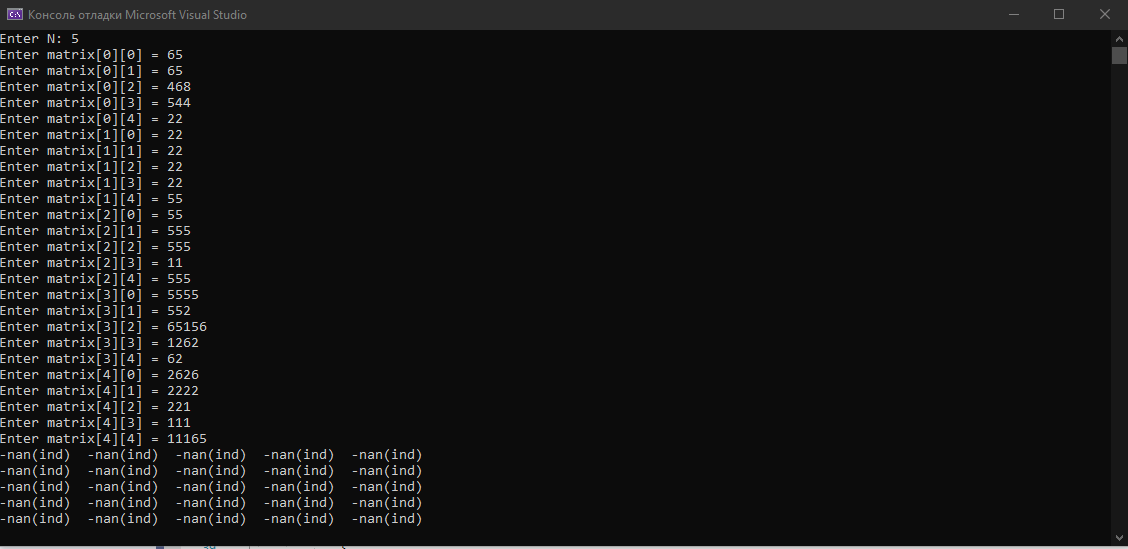
\includegraphics{skrin.png}

\label{sec:exp}

\begin{thebibliography}{9}
\bibitem{Knuth-2003}Кнут Д.Э. Всё про \TeX. \newblock --- Москва: Изд. Вильямс, 2003 г. 550~с.
\bibitem{Lvovsky-2003}Львовский С.М. Набор и верстка в системе \LaTeX{}. \newblock --- 3-е издание, исправленное и дополненное, 2003 г.
\bibitem{Voroncov-2005}Воронцов К.В. \LaTeX{} в примерах. 2005 г.
\end{thebibliography}

\end{document}